%
% Lösung.tex -- Beispiel-File für Lösung
%
% (c) 2020 Prof Dr Andreas Müller, Hochschule Rapperswil
%
% !TEX root = ../../buch.tex
% !TEX encoding = UTF-8
%
\section{Lösung
	\label{gezeiten:section:Lösung}}
\rhead{Lösung}
Die Lösung des Problems besteht aus zwei Teilen, der erste Teil besteht darin die Kurve des gemessenen Wasserstandes in Sinuswellen aufzuteilen, analog der Fourier Analyse.
Im zweiten Teil müssen lediglich die neun Sinuswellen miteinander addiert werden, um die Gezeiten vorherzusagen.
Die im Prozess erste Maschine entwickelte Lord Kelvin erst einige Jahre später als die Maschine, welche für den zweiten Schritt benötigt wird.

\subsection{Partialtiden}
Die Partialtiden sind die angesprochenen unterschiedlichen Frequenzkomponenten, welche benötigt werden für die Vorhersage der Gezeiten.
Bei den Partialtiden wird unterschieden zwischen täglichen, halbtäglichen und vierteltäglichen Gezeiten.
Die tägliche Gezeit tritt ungefähr ein Mal pro Tag ein, grob gesagt entsteht dabei einmal Ebbe und Flut pro Tag.
Bei der halbtäglichen Gezeit erscheint Ebbe und Flut je zwei Mal pro Tag, bei der vierteltäglichen Gezeit sind es dann bereits vier Mal pro Tag.
Die Amplituden unterscheiden sich je nach Standort, und Meeresgrund.
Die halbtagesgezeit des Mondes hat im Normalfall die höchsten Amplituden, gefolgt vom Hauptsonnenhalbtag.
Grundsätzlich kann gesagt werden, dass die halbtagesgezeiten die höchsten Amplituden aufzeigen, gefolgt von den täglichen Gezeiten.
Bei den vierteltäglichen Gezeiten sind die Amplituden, kleiner als zehn Zentimeter, die Auswirkungen sind daher fast gleich Null.
In der Tabelle \ref{gezeiten:tabelle:partialtiden} sind die wichtigsten Partialtiden abgebildet.
Je mehr Partialtiden verwendet werden, desto genauer würde die Vorhersage werden. 

\begin{table}
	\centering
	
\begin{tabular}{|l|l|r|r|r|r|c|r|r|}
	\hline
	Tide&Symbol&Zeit [h]&MICH&MS&PR&AK&CA&HALLO\\
	\hline \hline
	Halbtägige Mondtide&M$_{2}$&12.42&268.7&3.9&15.9&97.3&58.0&23.0\\
	\hline
	Halbtägige Sonnentide&S$_{2}$&12.00&42.0&3.3&2.1&32.5&13.7&9.2\\
	\hline
	Grösserer halbtägiger&&&&&&&&\\
	elliptischer Mond&N$_{2}$&12.66&54.3&1.1&3.7&20.1&12.3&4.4\\
	\hline
	Kleinere halbtägige&&&&&&&&\\
	elliptische Mondform&L$_{2}$&12.19&13.5&0.1&0.5&2.4&1.6&0.5\\
	\hline\hline 
	Hauptdeklination&K$_{1}$&23.93&15.6&16.2&9.0&39.8&36.8&16.7\\
	\hline
	Hauptmond&O$_{1}$&25.82&11.9&16.9&7.7&25.9&23.0&9.2\\
	\hline
	Hauptsonne&P$_{1}$&24.07&5.2&5.4&2.9&12.6&11.6&5.1\\
	\hline\hline
	Flachwasser des HM&M$_{4}$&6.21&6.0&0.6&-&0.9&2.3&-\\
	\hline
	Vierteltägliches FW&MS$_{4}$&6.10&1.8&-&-&0.6&1.0&-\\
	\hline	
\end{tabular}
	
\caption{In dieser Tabelle sind die neun wichtigsten Partialtiden aufgeführt. In der zweiten Spalte, wird die Periode in Stunden angegeben. Ab der vierten Spalte sind die Amplituden der Partialtiden in Zentimeter angegeben. Die Abkürzungen stehen für folgende Orte: MICH=Ostküste im Norden der USA; MS=Westküste der USA; PR=Puerto Rico (Insel zwischen Nord- und Südamerika; AK=Kodiak, Alaska; CA=San Francisco, California; HALLO= Hilo, Hawaii)}
\label{gezeiten:tabelle:partialtiden}
\end{table}

Lord Kelvin beobachtete damals über mehrere Jahre die Planeten und die Gezeiten um die in der \ref{gezeiten:tabelle:partialtiden} abgebildeten Werte herauszufinden. 

\subsection{Gezeitenkurve in Sinuswellen aufteilen
	\label{gezeiten:subsection:malorum}}
Wie bereits beschrieben musste Lord Kelvin eine Maschine erfinden, welche eine Gezeitenkurve in ihre Komponentfrequenzen zerlegt.
Diese Maschine entwickelte Lord Kelvin jedoch nicht alleine, sondern er zog sich die Hilfe seines älteren Bruders James Thompson bei.
Zusammen entwickelten sie die den mechanischen Integrator.
Die Funktionsweise wird nachfolgend beschrieben, um die funktionweise besser zu verstehen, ist in der Abbildung  \ref{fig: skizze-integralmaschine}eine Skizze zum mechanischen Integrator abgebildet.
Die Abbildung \ref{fig:harmonicanalyserdiscandsphere} zeigt eine Foto eines mechanischen Integrators.
Für diese Maschine benötigt er eine Scheibe, eine Welle, eine Kugel, ein Ausgabepapier für den Integral und natürlich die bestehende Wasserstandskurve.
Die Kugel wird dafür in der horizontalen Achse auf die Scheibe gelegt.
Je nach Position der Kugel, bewegt sich die kurve, langsam, schnell oder sogar rückwärts.
Die Bewegung der Kugel, wird über die Welle weitergegeben an das Ausgabepapier.
Bewegt sich die Kugel auf der Scheibe schnell, ist die Stammfunktion des Integrals in diesem Moment steiler.
Bewegt sich die Kugel auf der Scheibe langsam, sprich befindet sich diese nahe am Zentrum der Scheibe, entsteht ein flaches Integral.
Wenn sich die Kugel exakt im Zentrum befindet, entsteht auf dem Ausgabepapier ein Wendepunkt.
Um die Position der Kugel zu bestimmen, wird mit einem Stift die Wasserstandskurve nachgefahren, wobei der Stift mit der Kugel verbunden ist.
Die vorhandene Kurve ist dabei orthogonal zum ganzen Rest der Maschine.
Das Papier mit der vorhanden Kurve, bewegt sich also von unten nach oben.
Für das Integral mit der Sinuskurve lässt es sich mathematisch \[
a_k
=  
\int_0^{2\pi} R(t) \sin v_kt \, dt
\]
so darstellen.


\begin{figure}
	\centering
	\includegraphics[width=\textwidth]{"papers/gezeiten/Skizze Integralmaschine"}
	\caption{Skizze mechanischer Integrator}
	\label{fig:skizze-integralmaschine}
\end{figure}
% TODO: \usepackage{graphicx} required
\begin{figure}
	\centering
	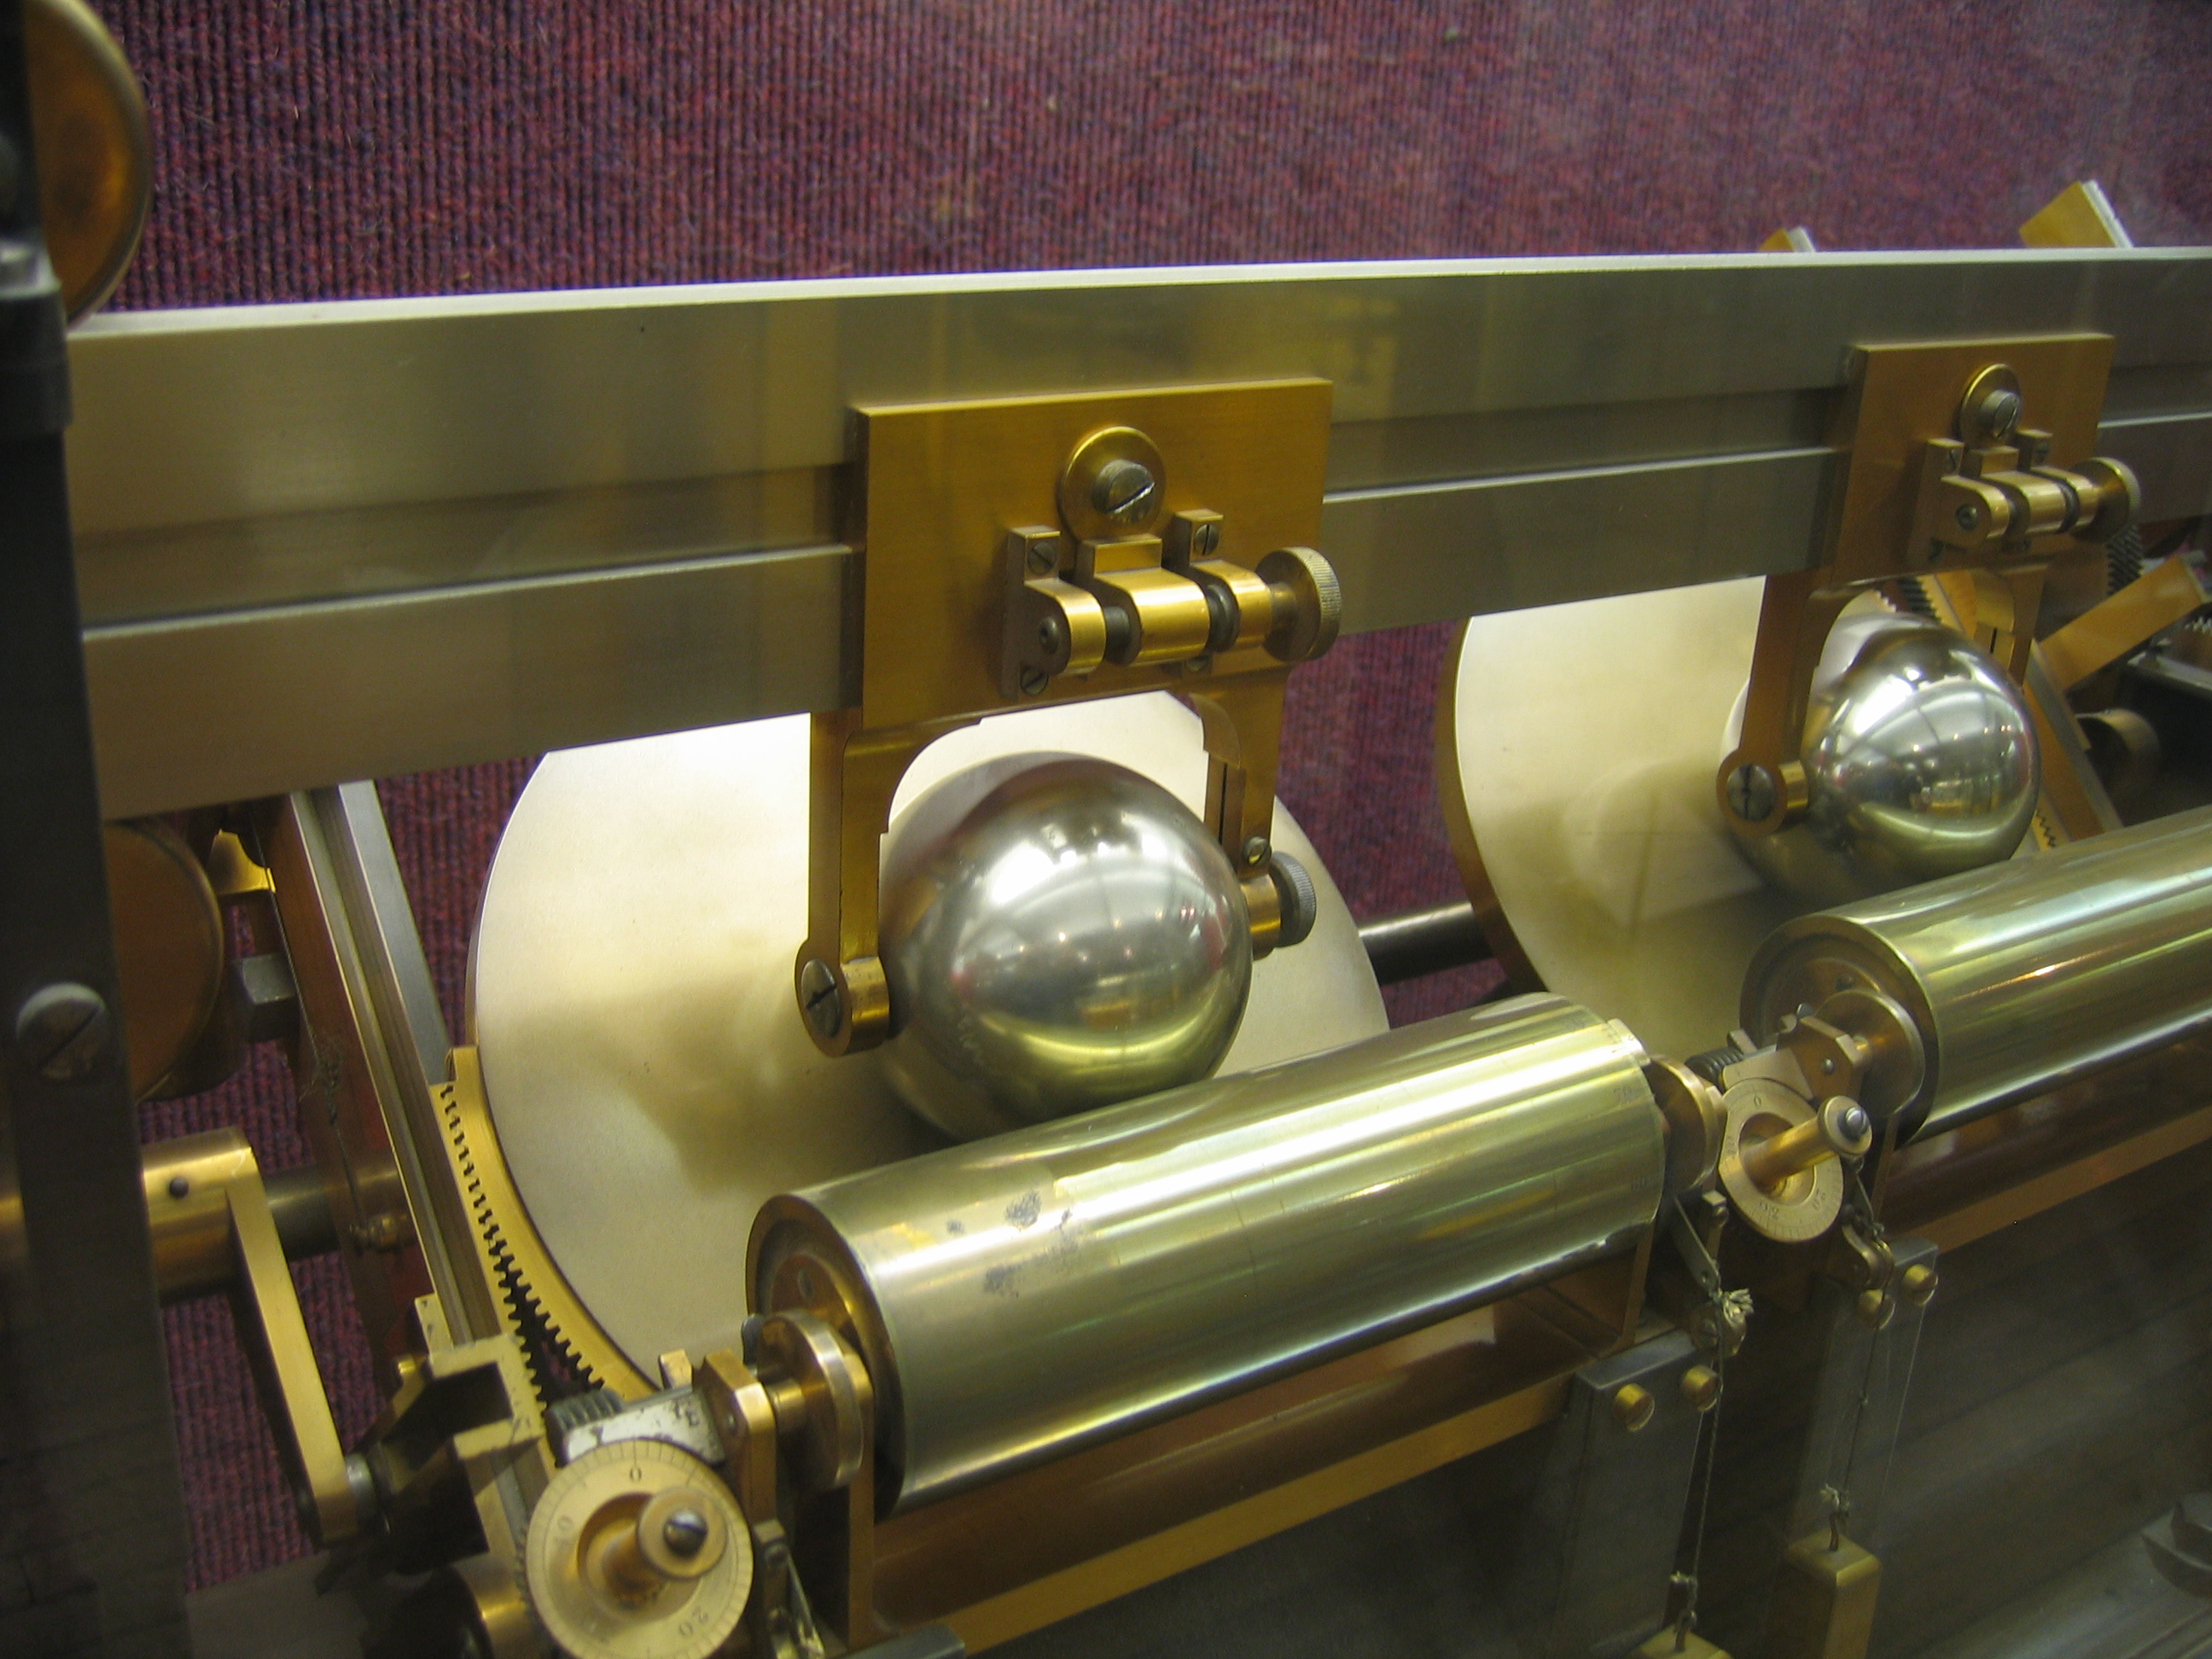
\includegraphics[width=\textwidth]{papers/gezeiten/Harmonic_analyser_disc_and_sphere}
	\caption{Kugel Scheiben Integrator (Quelle: \cite{gezeiten:KugelScheibenIntegrator }
	\label{fig:harmonicanalyserdiscandsphere}
\end{figure}

Für diesen Prozess, der Fourier Analyse, muss jedoch die  Wasserstandskurve als erstes mit der Sinuswelle mit der entsprechenden Frequenz mulitpliziert werden.
Um die Multiplikation in den Prozess zu integrieren, wird die Scheibe mit der Frequenz hin- und hergedreht.
Somit ist die Ausgabekurve das Integral, der Mulitplikation von der Sinuswelle mit der entsprechenden Funktion und der Wasserstandskuve, und somit schon das gewünschte Resultat.
Um den Koeffizienten zu erhalten, muss lediglich das entstandene Integral durch die Gesamtzeit geteilt werden.

Mathematisch kann dieser Vorgang folgendermassen beschrieben werden:
Mit dieser Analyse werden die Amplitude, sowie die Phase bestimmt.
Um die vorhandene Summenkurve, sprich die Aufzeichnung des Wasserstandes, zu zerlegen, wird sie in die standardisierte Form $H\cdot\cos(vt+p)$ gebracht.
Um auch die Phase zu erhalten, wird unter der Verwendung einer standardmässigen trigonometrischen Identität als $A\cdot\cos(vt)+B\cdot\sin(vt)$ umgeschrieben.
Dabei gilt $A=H\cdot\cos(\phi)$ und $B=-H\cdot\sin(\phi)$ und $v$ steht für die Geschwindigkeit, $t$ für die Zeit und $\phi$ für die Winkelgeschwindigkeit, respektive die Phase.
Dadurch erhält man am Ende aus der Aufzeichnung des Gezeitenpegels $R(t)$ die Kosinus- und die Sinusamplituden A und B für eine bestimmte Geschwindigkeit $v$.


\subsection{Sinuswellen addieren}

Um nun die erhaltenen Sinuswellen miteinander zu addieren, zog Lord Kelvin wiederum Hilfe bei.
Er wusste von einem Gerät mit dem Namen Scotch-Yoke.
Dieser Scotch Yoke konnte eine Sinusbewegung erzeugen, sprich aus einer Kreisbewegung wird eine Kurve.
Dieser Scotch Yoke besteht aus einem Rad, mit einem Zapfen.
Der Zapfen befindet sich dabei an der Peripherie des Rades.
Um den Zapfen befindet sich eine freibewegende Öse, in der breite des Rades, damit die vertikalen Bewegungen des Zapfens festgehalten werden könnnen.
Dieser Scotch Yoke kann also die Sinusbewegungen aufzeichnen, und ist in \ref{fig:scotch-yoke}
Seine Herausforderung war es jedoch, mindestens neun solche Sinuswellen miteinander zu addieren.
Den Input für die Lösung bekam er seinem Freund Mr. Tower, welcher er zufälligerweise im Zug traf und ihm da das Problem schilderte.
Towers schlug ihm vor, eine Kette, welche um mehrere Rollen läuft, zu verwenden, wie Wheatstone in seinem alphabetischen Telegrapheninstrument.
Dies war der entscheidende Input für Lord Kelvin, er skizzierte sogleich, die erste Gezeitenvorhersage Maschine. Seine Skizze könnte vereinfacht etwa so ausgesehen haben, wie die Skizze in der Abbildung \ref{fig:skizze-maschine}.
Wie Skizze für die dritte Gezeitenvorhersagemaschine ausgesehen hat, ist in der \ref{fig:thompson-skizze} ersichtlich. 
Und zwar befestigte er an jedem Scotch-Yoke ein Rad.
Dort wo Wheatstone eine Kette verwendete, verwendete Lord Kelvin einen Draht, welcher am Anfang befestigt ist.
Und danach durch alle Rädchen der Scotch-Yokes hindurchläuft.
Am Ende des Drahts befestigte er ein Gewicht und einen Stift.
So konnte er alle Beträge der Sinuswellen mit den unterschiedlichen Frequenzen auf einmal addieren, und erhielt so die Kurve für die Vorhersage der Gezeiten.

\begin{figure}
	\centering
	\caption{Darstellung eines Scotch Yoke(Quelle: \cite{gezeiten:Yoke)}
	\label{fig:scotch-yoke}
	\includegraphics[width=\textwidth]{"papers/gezeiten/Scotch Yoke"}
\end{figure}

\begin{figure}
	\centering
	\includegraphics[width=\textwidth]{"papers/gezeiten/Skizze Maschine"}
	\caption{Skizze der Gezeitenvorhersage Maschine}
	\label{fig:skizze-maschine}
\end{figure}

\begin{figure}
	\centering
	\includegraphics[width=\textwidth]{"papers/gezeiten/Thompson Skizze"}
	\caption{Vollumfängliche Skizze der 3. Gezeitenvorhersagemaschine von Lord Kelvin(Quelle: \cite{gezeiten:Thompson)}
	\label{fig:thompson-skizze}
\end{figure}

Wenn man nun alle relativen Beträge der unterschiedlichen Frequenzkörper kennt, kann mit dieser Maschine ziemlich einfach die Gezeitenvorhersage gemacht werden.
Dies war ein grosser Sprung der Technik.
Wenn nun Lord Kelvin oder auch jemand anders, vier Stunden den Hebel der Maschine betätigte, wurde die Gezeitenvorhersage für ein ganzes Jahr mechanisch gerechnet.
Nun konnte mit einer Scotch-Yoke-Riemenmaschine, viel einfacher die Gezeitenvohersage gemacht werden.

In der Mathematik wird die Vorhersage der Gezeiten harmonische Analyse genannt.
Die Vorhersage der Gezeiten für einen bestimmten Hafen wird mit $Z_0+\sum A_k\cdot\cos(v_kt+\phi_k)$ wobei $Z_0$ die durschnittliche Höhe des Wasserstandes im Hafen ist. Die Zahlen $A_k$, $v_k$, $t$ und $\phi_k$ sind die Amplitude in cm, die Geschwindigkeit Grad/Stunde, Zeit in Stunden und die Phase in Grad angegeben.
Kurz kann auch gesagt werden: Die einzelnen harmonischen Schwingungen der Partialtiden werden übereinandergelegt, damit am Ende wieder eine Wasserstandskurve entsteht.

Diese Präzisionsmaschinen wurden bis in die 1960er Jahre verwendet, und fanden auch im zweiten Weltkrieg grossen Anklang.
Später wurden die Maschinen mit zusätzlichen Frequenzkomponenten erweitert.
So entstand unter anderem der grösste Gezeitenrechner mit 62 unterschiedlichen Frequenzen.
Seit Jahrzehnten stand im deutschen Schifffahrtsmuseum ein Gezeitenrechner, welcher aber ungenutzt blieb und somit verstaubte
Im Jahre 2020 wurde der älteste deutsche Gezeitenrechner aus dem Jahr 1915 restauriert.
Dies war eine kostspielige Sache, die ganze Restauration kostete 50'000 Euro.
Die tausenden Einzelteile wurden zerlegt, gereinigt und wieder zusammengebaut.
Das war eine grosse Herausforderung, denn es existieren keine Baupläne.

Im Zeitalter der digitalen Computer werden die mechanischen Gezeitenrechner also nur noch im Museum verwendet.
Für die Schiffahrt oder auch für das Bauingenieurwesen, werden die Berechnungen heute digital mit dem Computer durchgeführt, diese sind präziser, zuverlässiger und schneller, denn die genauen Einstellungen beim analogen Gezeitenrechner waren, und sind immer noch sehr kompliziert.
